%%%%%%%%%%%%%%%%%%%%%%%%%%%%%%%%%%%%%%%%%
% Programming/Coding Assignment
% LaTeX Template
%
% This template has been downloaded from:
% http://www.latextemplates.com
%
% Original author:
% Ted Pavlic (http://www.tedpavlic.com)
%
% Note:
% The \lipsum[#] commands throughout this template generate dummy text
% to fill the template out. These commands should all be removed when 
% writing assignment content.
%
% This template uses a Perl script as an example snippet of code, most other
% languages are also usable. Configure them in the "CODE INCLUSION 
% CONFIGURATION" section.
%
%%%%%%%%%%%%%%%%%%%%%%%%%%%%%%%%%%%%%%%%%

%----------------------------------------------------------------------------------------
%	PACKAGES AND OTHER DOCUMENT CONFIGURATIONS
%----------------------------------------------------------------------------------------

\documentclass{article}

\usepackage{fancyhdr} % Required for custom headers
\usepackage{lastpage} % Required to determine the last page for the footer
\usepackage{extramarks} % Required for headers and footers
\usepackage[usenames,dvipsnames]{color} % Required for custom colors
\usepackage{graphicx} % Required to insert images
\usepackage{listings} % Required for insertion of code
\usepackage{courier} % Required for the courier font
\usepackage{lipsum} % Used for inserting dummy 'Lorem ipsum' text into the template
\usepackage{paralist}
\usepackage{hyperref}

% Margins
\topmargin=-0.45in
\evensidemargin=0in
\oddsidemargin=0in
\textwidth=6.5in
\textheight=9.0in
\headsep=0.25in

\linespread{1.1} % Line spacing

% Set up the header and footer
\pagestyle{fancy}
\lhead{\hmwkAuthorName} % Top left header
\chead{\hmwkClass: \hmwkTitle} % Top center head
\rhead{\firstxmark} % Top right header
\lfoot{\lastxmark} % Bottom left footer
\cfoot{} % Bottom center footer
\rfoot{Page\ \thepage\ of\ \protect\pageref{LastPage}} % Bottom right footer
\renewcommand\headrulewidth{0.4pt} % Size of the header rule
\renewcommand\footrulewidth{0.4pt} % Size of the footer rule

\setlength\parindent{0pt} % Removes all indentation from paragraphs

%----------------------------------------------------------------------------------------
%	CODE INCLUSION CONFIGURATION
%----------------------------------------------------------------------------------------

\definecolor{MyDarkGreen}{rgb}{0.0,0.4,0.0} % This is the color used for comments
\definecolor{MyDarkRed}{rgb}{0.4,0.0,0.0}
\lstset{language=Ruby, % Use Perl in this example
        basicstyle=\small\ttfamily, % Use small true type font
        keywordstyle=[1]\color{Blue}\bf, % Perl functions bold and blue
        keywordstyle=[2]\color{Purple}, % Perl function arguments purple
        keywordstyle=[3]\color{Blue}\underbar, % Custom functions underlined and blue
        identifierstyle=, % Nothing special about identifiers                                         
        commentstyle=\usefont{T1}{pcr}{m}{sl}\color{MyDarkGreen}\small, % Comments small dark green courier font
        stringstyle=\color{MyDarkRed}, % Strings are red
        showstringspaces=false, % Don't put marks in string spaces
        tabsize=5, % 5 spaces per tab
        %
        % Put standard Perl functions not included in the default language here
        morekeywords={rand},
        %
        % Put Perl function parameters here
        morekeywords=[2]{on, off, interp},
        %
        % Put user defined functions here
        morekeywords=[3]{test},
       	%
        morecomment=[l][\color{Blue}]{...}, % Line continuation (...) like blue comment
}


% Creates a new command to include a perl script, the first parameter is the filename of the script (without .pl), the second parameter is the caption
\newcommand{\perlscript}[2]{
\begin{itemize}
\item[]\lstinputlisting[caption=#2,label=#1]{#1.pl}
\end{itemize}
}

%----------------------------------------------------------------------------------------
%	DOCUMENT STRUCTURE COMMANDS
%	Skip this unless you know what you're doing
%----------------------------------------------------------------------------------------

% Header and footer for when a page split occurs within a problem environment
\newcommand{\enterProblemHeader}[1]{
\nobreak\extramarks{#1}{#1 continued on next page\ldots}\nobreak
\nobreak\extramarks{#1 (continued)}{#1 continued on next page\ldots}\nobreak
}

% Header and footer for when a page split occurs between problem environments
\newcommand{\exitProblemHeader}[1]{
\nobreak\extramarks{#1 (continued)}{#1 continued on next page\ldots}\nobreak
\nobreak\extramarks{#1}{}\nobreak
}

\setcounter{secnumdepth}{0} % Removes default section numbers
\newcounter{homeworkProblemCounter} % Creates a counter to keep track of the number of problems

\newcommand{\homeworkProblemName}{}
\newenvironment{homeworkProblem}[1][Problem \arabic{homeworkProblemCounter}]{ % Makes a new environment called homeworkProblem which takes 1 argument (custom name) but the default is "Problem #"
\stepcounter{homeworkProblemCounter} % Increase counter for number of problems
\renewcommand{\homeworkProblemName}{#1} % Assign \homeworkProblemName the name of the problem
\section{\homeworkProblemName} % Make a section in the document with the custom problem count
\enterProblemHeader{\homeworkProblemName} % Header and footer within the environment
}{
\exitProblemHeader{\homeworkProblemName} % Header and footer after the environment
}

\newcommand{\problemAnswer}[1]{ % Defines the problem answer command with the content as the only argument
\noindent\framebox[\columnwidth][c]{\begin{minipage}{0.98\columnwidth}#1\end{minipage}} % Makes the box around the problem answer and puts the content inside
}

\newcommand{\homeworkSectionName}{}
\newenvironment{homeworkSection}[1]{ % New environment for sections within homework problems, takes 1 argument - the name of the section
\renewcommand{\homeworkSectionName}{#1} % Assign \homeworkSectionName to the name of the section from the environment argument
\subsection{\homeworkSectionName} % Make a subsection with the custom name of the subsection
\enterProblemHeader{\homeworkProblemName\ [\homeworkSectionName]} % Header and footer within the environment
}{
\enterProblemHeader{\homeworkProblemName} % Header and footer after the environment
}

%----------------------------------------------------------------------------------------
%	NAME AND CLASS SECTION
%----------------------------------------------------------------------------------------

\newcommand{\hmwkTitle}{Enhancing the CS-Alumni Application} % Assignment title
\newcommand{\hmwkDueDate}{Monday,\ December\ 10,\ 2012} % Due date
\newcommand{\hmwkClass}{SE31520} % Course/class
\newcommand{\hmwkAuthorName}{Alexander Brown} % Your name

%----------------------------------------------------------------------------------------
%	TITLE PAGE
%----------------------------------------------------------------------------------------

\title{
\vspace{2in}
\textmd{\textbf{\hmwkClass:\ \hmwkTitle}}\\
\normalsize\vspace{0.1in}\small{Due\ on\ \hmwkDueDate}\\
%\vspace{0.1in}\large{\textit{\hmwkClassInstructor\ \hmwkClassTime}}
\vspace{3in}
}

\author{\textbf{\hmwkAuthorName}}
\date{} % Insert date here if you want it to appear below your name

%----------------------------------------------------------------------------------------

\begin{document}

\maketitle

%----------------------------------------------------------------------------------------
%	TABLE OF CONTENTS
%----------------------------------------------------------------------------------------

%\setcounter{tocdepth}{1} % Uncomment this line if you don't want subsections listed in the ToC

\newpage
\tableofcontents
\newpage


%----------------------------------------------------------------------------------------
\section{Introduction}
%----------------------------------------------------------------------------------------
The CS-Alumni (CSA) Application prototype is a Ruby on Rails application which runs as a
web service. It supports browser-based interaction as well as some RESTful interaction.
The purpose of this project is to increase the capabilities of the CSA Application (to
prevent confusion I will now refer to it as the CSA server) so it can support a 
desktop-based client (which I will refer to as the CSA client).

In recent years REST interoperability has increased in popularity and prevalence and, for
this sort of project, REST is the best technique for the job. Other methods of 
interoperability like sockets of RPC would be too heavyweight for purpose, and would just
complicate the interaction between client and server.

REST allows a lot of code reuse in the server, especially with Ruby on Rails which has 
nice ideas about routing and responding formats. As Rails uses all forms of REST requests
under the covers, not just the ones supported by browsers, it makes the change from a 
web-based application to a RESTful service very easy (in fact a lot of it has already 
been done).

The only thing I really anticipate having to do to the server is expose a little more 
information for more complex operations such as logging-in or checking access. As these
operations are not handled in a RESTful way to make using the web-based version sane 
(i.e. using sessions to persist log-in credentials).

The only thing the client will need to do is expose REST requests in a nice format to
non-technical users. Of course this will also expose the server to other potential 
clients other than the one discussed here. But again this is not a bad thing, so long as
security is maintained. An example of this is a technical user using cURL to issue REST
requests via a shell.


\clearpage
%----------------------------------------------------------------------------------------
\section{Server Architecture}
\label{sec:server}
%----------------------------------------------------------------------------------------
Having worked in a Level 3 Service team, my attitude toward changing existing code is not
to do so unless it is completely necessary and at that, to modify the code as little as
possible.

The first change I made was to make a simple addition to the UserController which would
echo the username of the currently logged-in user. This allowed me to
\begin{inparaenum}[\itshape a\upshape)]
\item confirm the user has been logged-in;
\item check if the user is an administrator (currently this is defined by the username
being equal to ``admin'').
\end{inparaenum}

This change involved adding a single method (and associated \verb$GET$ route) which only rendered
JSON (i.e. it would only accept content-type JSON).

The only other change I made to add functionality to include the details of a user's
image in the JSON file from the \verb$GET$ request to \verb$/user/:id.json$. 

Figure~\ref{fig:server-uml-class} shows the overall class diagram for the CSA Server.

\begin{figure}[h]
\centering
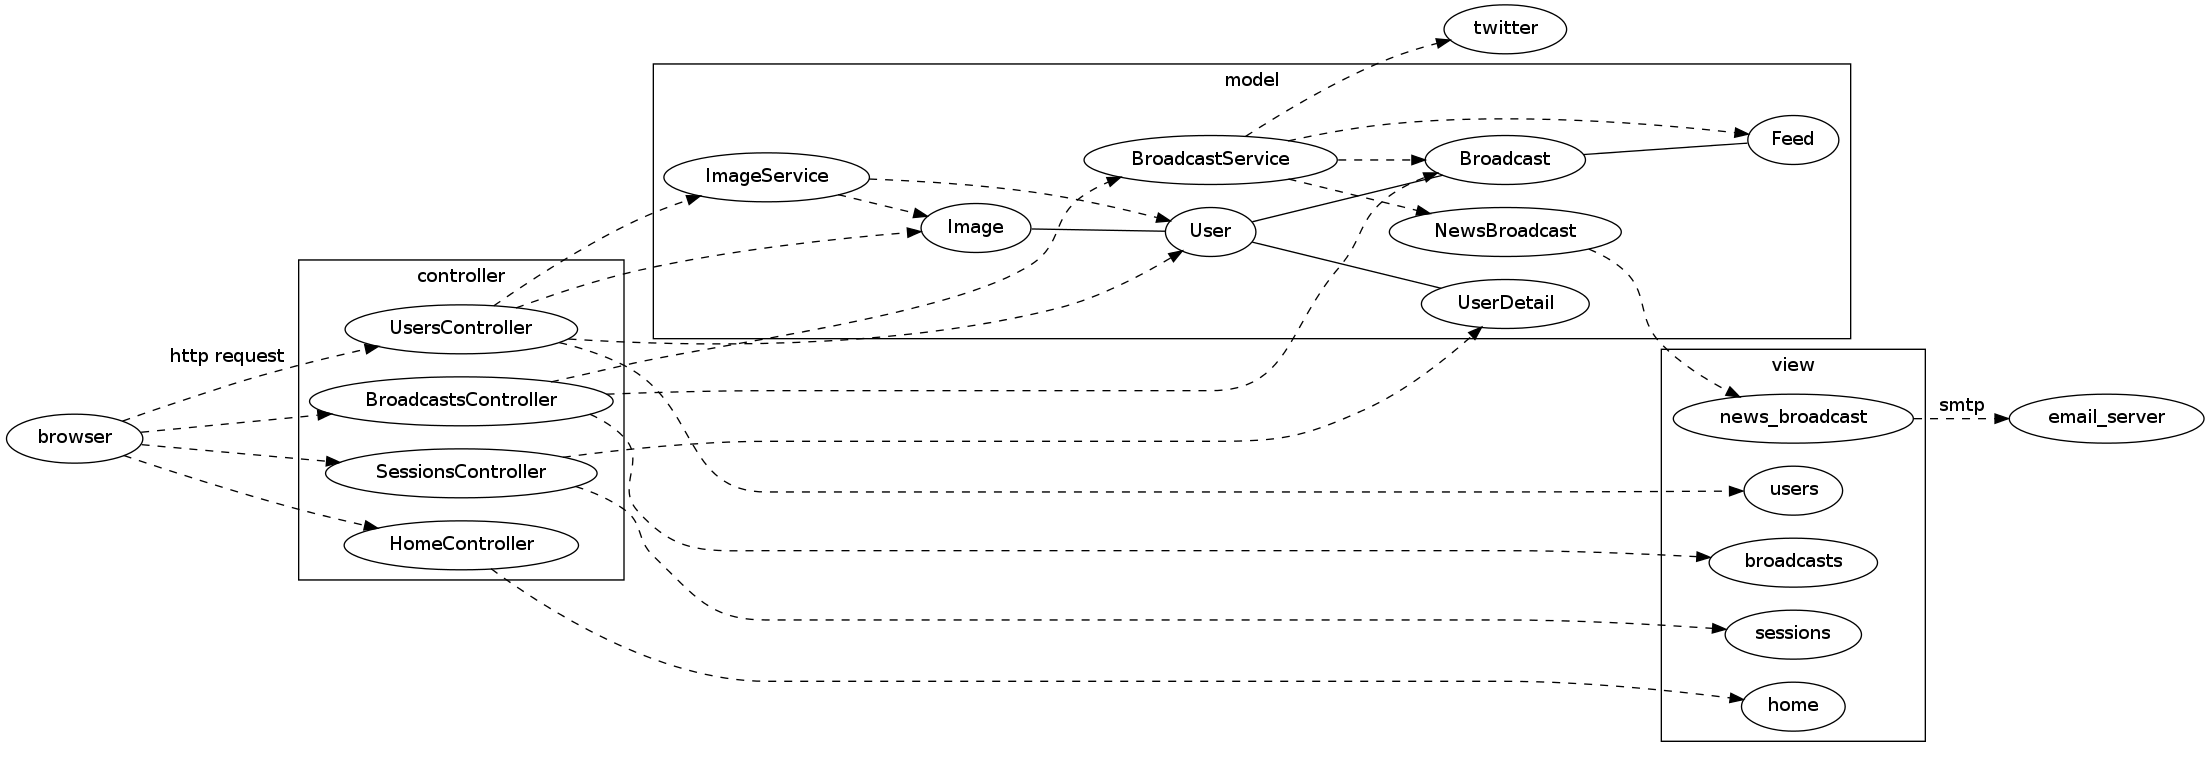
\includegraphics[width=.95\textheight, angle=90]{img/server-uml-class.png}
\caption{Class diagram for the CSA server}
\label{fig:server-uml-class}
\end{figure}

As is apparent from figure~\ref{fig:server-uml-class}, the architecture of the server
hasn't changed at all. The only additions are those mentioned above (the addition of a
single \verb$GET$ route, and some additional information in the User's JSON file). Other
than this I felt no real need to change the architecture of the server, nor the way in
which it performs the current functionality.

I did have to fix some small pieces of code in the way emails were produced and sent to
make that code actually work. This was part of fixing the tests on the CSA server.

\clearpage
%----------------------------------------------------------------------------------------
\section{Client Architecture}
%----------------------------------------------------------------------------------------
As the client doesn't need to do a lot I decided to keep it fairly simple. I still tried
to follow the Model, View, Controller (MVC) design pattern as best as I could. Separating
out a lot of the REST interaction into a sole class.

This also means it would be relatively easy to swap out this method of interaction 
without too much effort.

The views take up the majority of the class diagram as there are different ways of 
presenting the same information. However even these have been kept as simple as possible.

Figure~\ref{fig:client-uml-class} shows the UML Class diagram for the client.

\begin{figure}[h]
\centering
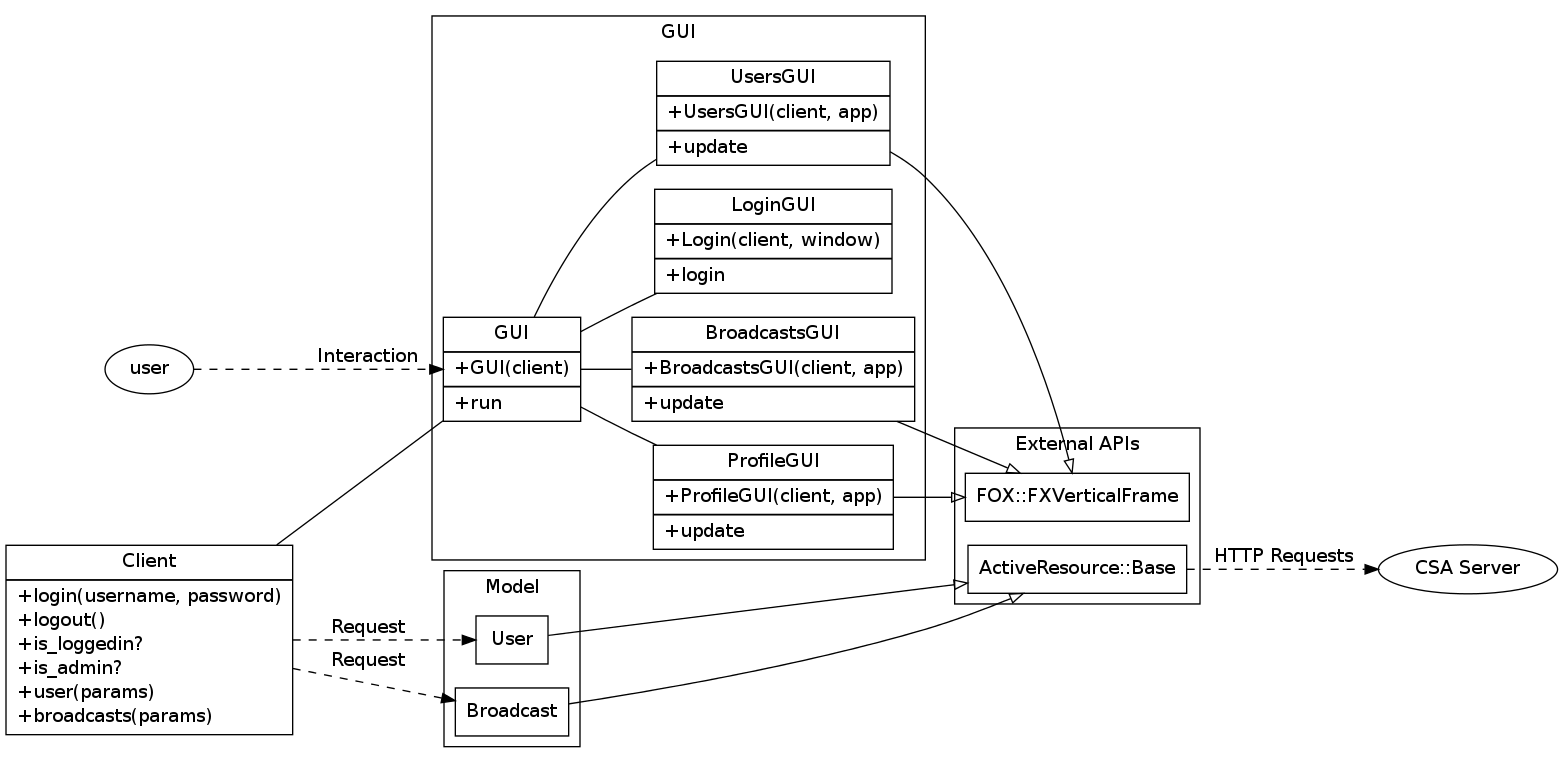
\includegraphics[width=.9\textheight, angle=90]{img/client-uml-class.png} 
\caption{UML Class diagram for the client}
\label{fig:client-uml-class}
\end{figure}

From this I then started to consider the choice of language. Ruby was the obvious choice
to keep a bit of compatibility between client and server. I also found that Rails has a
gem which provides client-based REST access to a Rails application; ActiveResource. This
saved me a lot of time and effort during implementation, not having to work out the 
exact, correct, REST requests and the form the JSON files passed between the two take.

Ruby also has some nice graphics libraries, FXRuby is one which is cross-platform, with a
lot of good documentation, based on the FOX toolkit for C++.

\clearpage
%----------------------------------------------------------------------------------------
\section{Test Strategy}
%----------------------------------------------------------------------------------------
The first part of the strategy was to fix all the failing tests on the CSA server; the 
most of these were caused by there not being a logged-in user when performing the 
actions. It was a simple matter of creating an entry in the \verb$user_details$ table in
the test fixtures. I then got this entry and added it to a fake session Rails testing
provides to assist with this scenario.\cite{buren07}

With this the majority of the failing tests then passed. The only other broken tests
concerned emailing out broadcasts. This was caused by a problem with the code to do this,
as mentioned in the \nameref{sec:server}~section.

With this complete I then turned my attention to testing the CSA client. However, when
I started to work out what needed testing I found out there was very little. It seemed
pointless to test the ActiveResource models in the client as they were provided by an
external API which should be well tested. The only thing I could test is that the methods
for logging-in and checking administrator users to make sure the GUI only enables the
correct options.

The final step was to look back at the server. As all the client does is poll the server
for information using ActiveResrouce it stands to reason that if the server is correctly
tested, the client should work correctly with it. Of course in real life it's never quite
that simple, but just running and using the client should be enough to verify that it's
working correctly.

\clearpage
%----------------------------------------------------------------------------------------
\section{Evaluation}
%----------------------------------------------------------------------------------------
I found this assignment quite easy in terms of programming. Having spent a year in 
industry; especially in a role which involved heavily interacting with existing systems
and external APIs; this was all old hat to me. I had also taken some time during my year
to look and play with Diaspora - a decentralised social network platform written in Ruby
on Rails, so I was somewhat familiar with some of the technologies involved too.

I very quickly mastered FXRuby; again I have spent quite a bit of time playing with 
graphics libraries so picking up a new one which has parallels to Java's SWT, was a 
fairly easy task; and produced a quick mock up of the GUI I would be using for the Client
in a single class. I then abstracted out some of the resources into separate classes 
where appropriate.

The biggest difficulty I had on this assignment was when it came to updating a user's
profile from the client. Because of the way ActiveResource works it sends every single 
detail about a model object back through the \verb$PUT$ request. This in turn caused the
server too result in a HTTP 500 error code as ActiveRecord was trying to update protected
attributes such as the \verb$id$, \verb$created_at$ and \verb$updated_at$ attributes.

Figure~\ref{fig:activeresource-to-activerrecord-500} shows the details of the request.

\begin{figure}[h]
\begin{verbatim}
PUT /users/41.json HTTP/1.1
Content-Type: text/json
Accept: text/json
... HTTP Authentication headers.
\end{verbatim}
\begin{lstlisting}[language=java]
{
  "created_at":"2012-11-05T14:27:03Z",
  "email":"cwl39@aber.ac.uk",
  "firstname":"Firstname39",
  "grad_year":1985,
  "id":41,
  "jobs":true,
  "phone":"01970 622422",
  "surname":"Test",
  "updated_at":"2012-12-02T12:25:56Z",
  "image":{
    "id":1,
    "photo_content_type":"image/jpeg",
    "photo_file_name":"P1210623.JPG",
    "photo_file_size":2087613,
    "photo_updated_at":"2012-08-13T11:14:04Z",
    "user_id":41
  }
}
\end{lstlisting}
\caption{Example of a PUT request to user with ID of 41}
\label{fig:activeresource-to-activerrecord-500}
\end{figure}

Digging a little deeper into this issue and looking through the log-files Rails produces
it turned out the ImageService class was receiving the Hash generated from the JSON file
and putting it straight into the User object. This was then causing ActiveRecord to fail
validations for changing protected values and returning a HTTP 500 error code to the 
request.

I tried filtering out the protected attributes using 
\verb$ActiveRecord.protected_attributes$, however this seemed to only contain certain 
attributes and not a whole list. I resolved this by iterating the hashes keys and seeing 
if \verb$ActiveRecord.available_attributes$ contained that key. If not it was removed 
from the hash. This fixed the problem and didn't cause any other problems. I had also 
tried nullifying the attributes client side, but this meant ActiveResource sent the 
request to the wrong place (as it lost the ID to guide it).

\clearpage
%----------------------------------------------------------------------------------------
\bibliographystyle{ieeetr}
\bibliography{se315}

\end{document}
